The program consists of six main classes:
\begin{enumerate}
    \item SortedQgram, which creates a table to index every sorted q-gram of given $ScoreClass$ and $q$.
    \item MultisetEncoder, which creates a table to encode every possible sorted q-gram to integer.
    \item Distribution, which approximates a threshold $k$ for a $k$-environment given a $ScoreClass$.
    \item QgramEnvironment, which generates a score matrix between all sorted $q$-grams and unsorted $q$-grams.
    \item SpacedSeedEncoder, which generate schemes to divide spaced seed, divides them into sub-$q$-grams and encodes them into sorted $q$-gram codes.
    \item CompositeEnvironment, which is the main class. It passes sequences into SpacedSeedEncoder, uses the sorted $q$-gram codes to call individual $k$-environment and generates a Cartesian product from the environments.
\end{enumerate}
In Figure~\ref{fig:classes}, the relationship and dataflow between the classes are outlined.

\begin{figure}[t]
\begin{center}
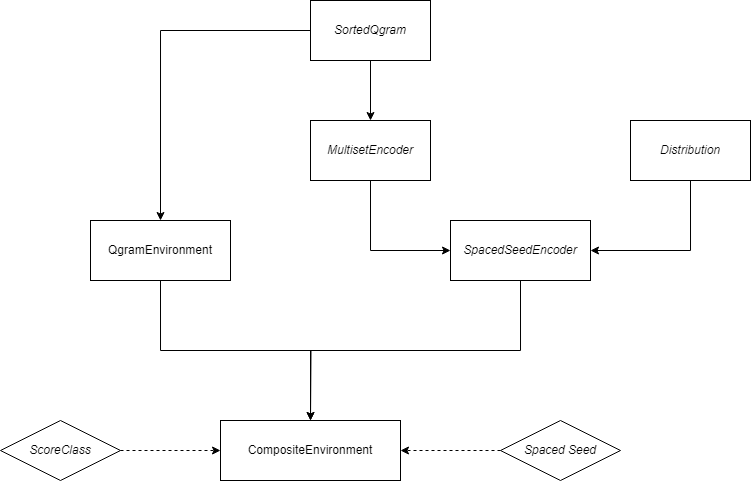
\includegraphics[scale=0.6]{graphics/Class Diagram.png}
\end{center}
\caption{Relationship between the six main classes and inputs. $Italic$ denotes compile-time evaluated classes.}
\label{fig:classes}
\end{figure}